\newpage
\subsection{Connecting your classes}
\texHeader
\hypertarget{static:references tex}{}

\begin{itemize}

\item[$\blacktriangleright$] Now, lets add some references. MOSL supports two reference types - a \emph{contained reference} and a \emph{simple reference}. Both
automatically update the other element involved in the reference automatically, which means you only have to declare a direction once.

\item[$\blacktriangleright$] Activate the \texttt{Card} editor and add a simple reference named \texttt{cardContainer} with a multiplicity of zero to one, of
type \texttt{Partition} (Fig.~\ref{fig:cardReference}). This means that a single card can belong to a maximum of 1 partition.

\begin{figure}[htbp]
	\centering
  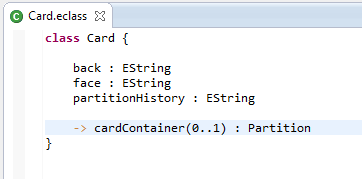
\includegraphics[width=0.5\textwidth]{eclipse_cardReference}
	\caption{Creating a \emph{simple reference} in Card}
	\label{fig:cardReference}
\end{figure} 

\item[$\blacktriangleright$] Now add a \emph{container reference} to \texttt{Partition}. Name it \texttt{card}, and allow it to hold an unlimited amount of
cards.

\item[$\blacktriangleright$] Congratulations, you have just built your first \emph{Bidirectional EReference}! In essence, you have now set up a relation that
allows a potentially infinite amount of item \texttt{card} to be stored in a cardContainer (partition), and restricts that \texttt{containedCard} to only
\emph{one} partition.

\item[$\blacktriangleright$] Now, lets create another bidirectional reference between \texttt{Partition} and \texttt{Box}. If you think about it, it's really
not all that different than the relation between \texttt{Partition} and \texttt{Card}. In fact, it's not different at all! A \texttt{Box} should be able to hold
an unlimited amount of partitions, but a \texttt{Partition} should only be allowed to belong to zero or one boxes. Name the two new relations
\texttt{containedPartition}, and \texttt{box}.

\item[$\blacktriangleright$] Your classes should now closely resemble Fig.~\ref{fig:allReferences}.

\item[$\blacktriangleright$] The next step is to set up two relations between \texttt{Partition} and itself, so it can shift between the previous and next
partition in the box. Create two new simple references, named \texttt{previous}, and \texttt{next}. Allow them to have a maximum of 1 link each. If you've done
everything correctly, your \texttt{Partition} class should now resemble Fig.~\ref{fig:partitionReferences}.

\item[$\blacktriangleright$] All of our references are now set up! To see how all of this is depicted visually, check out Fig.~\ref{fig:ereferences_all} in
\hyperlink{sec:static vis}{section 2.1}.

\newpage

\begin{figure}[htbp]
	\centering
  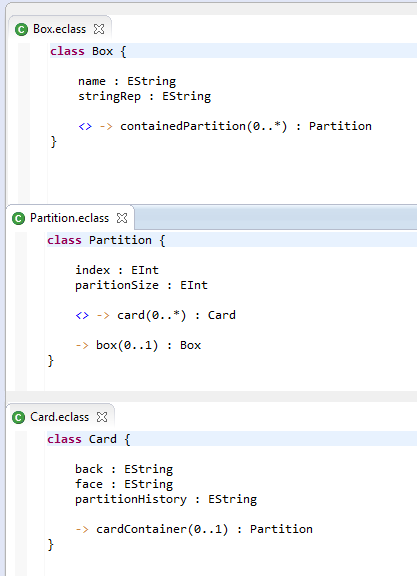
\includegraphics[width=0.5\textwidth]{eclipse_workspaceReferences}
	\caption{The Completed Bidirectional EReferences}
	\label{fig:allReferences}
\end{figure} 

\vspace{2cm}

\begin{figure}[htbp]
	\centering
  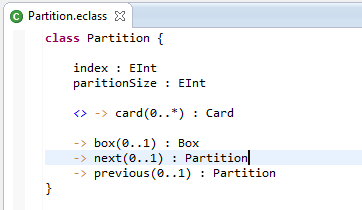
\includegraphics[width=0.5\textwidth]{eclipse_partitionReferences}
	\caption{All references in \texttt{Partition}}
	\label{fig:partitionReferences}
\end{figure} 

\fancyfoot[R]{$\triangleright$ \hyperlink{static:methods tex}{Next}}
\end{itemize}
